%%#! latex

%%%%%%%%%%             Preamble                   %%%%%%%%%%

\documentclass[12pt,dvipdfmx]{jarticle}
\usepackage{amsfonts,amssymb,amsmath,amscd,amsthm,latexsym}
\usepackage{graphicx}
\usepackage{fancybox}
\usepackage{okumacro}
%\usepackage{hyperref}
%\usepackage{showkeys}
%\usepackage{fancybox,ascmac}
%\usepackage{fancyhdr}
\pagestyle{empty}

\usepackage{hyperref}
\usepackage{bookmark}
\usepackage{pdfpages}

% pdfの栞の字化けを防ぐ
\AtBeginDvi{\special{pdf:tounicode EUC-UCS2}}

%%%%%%%%%%             Layout                     %%%%%%%%%%

\setlength{\topmargin}{-1cm}
\setlength{\textheight}{25cm}
\setlength{\textwidth}{16.5cm}
%\setlength{\oddsidemargin}{0cm}
%\setlength{\evensidemargin}{0cm}
%\addtolength{\textwidth}{.815in}
\addtolength{\oddsidemargin}{-2cm}
\addtolength{\evensidemargin}{-2cm}


%%%%%%%%%%             Macro (by Nasu)           %%%%%%%%%%

\renewcommand{\theenumi}{\arabic{enumi}}
\renewcommand{\theenumii}{\alph{enumii}}
\renewcommand{\theenumiii}{\roman{enumiii}}
\renewcommand{\labelenumi}{(\theenumi)}
\renewcommand{\labelenumii}{(\theenumii)}
\renewcommand{\labelenumiii}{[\theenumiii]}
%\renewcommand{\baselinestretch}{1.2}
%\renewcommand{\abstractname}{\sc Abstract}

%%%%%%%%%%           Commutative diagram          %%%%%%%%%%

% A litte smaller diagram than AMS CD envrionment

\newcommand{\mapright}[1]{%
\smash{\mathop{%
\hbox to 1cm{\rightarrowfill}}\limits^{#1}}}
\newcommand{\mapleft}[1]{%
\smash{\mathop{%
\hbox to 1cm{\leftarrowfill}}\limits^{#1}}}
\newcommand{\mapdown}[1]{\Big\downarrow
\llap{$\vcenter{\hbox{$\scriptstyle#1\,$}}$ }}
\newcommand{\mapup}[1]{\Big\uparrow
\rlap{$\vcenter{\hbox{$\scriptstyle#1$}}$ }}


%%%%%%%%%%            Text Start                 %%%%%%%%%%

\begin{document}

\begin{center}
 {\bf \Huge 東海大学理学部数学・情報数理談話会}
\end{center}

{\Large 以下の要領において談話会を開催致します. 多数の方の御来聴をお待ち致しております. 
\begin{tabbing}
\hspace{2.5cm} \=  \\
\noindent
日時 \> 2026年11月13日(金) \\
\> 15:20--16:05(前半), 16:20--17:05(後半) \\
\noindent
会場 \> 東海大学湘南校舎18号館7階 18-730 (情報数理ゼミ室10) \\
\noindent
講演者 \> 板井昌典氏(東海大学名誉教授) \\
\noindent
タイトル \> Tsimerman の業績とモデル理論 \\
\end{tabbing}

\noindent
アブストラクト: 別紙(次頁)参照

\begin{flushright}
  世話人: 那須 弘和\\
  nasu@tokai.ac.jp
\end{flushright}
}

\bookmark[page=1,level=0]{案内}
\bookmark[page=2,level=0]{アブストラクト}

\newpage

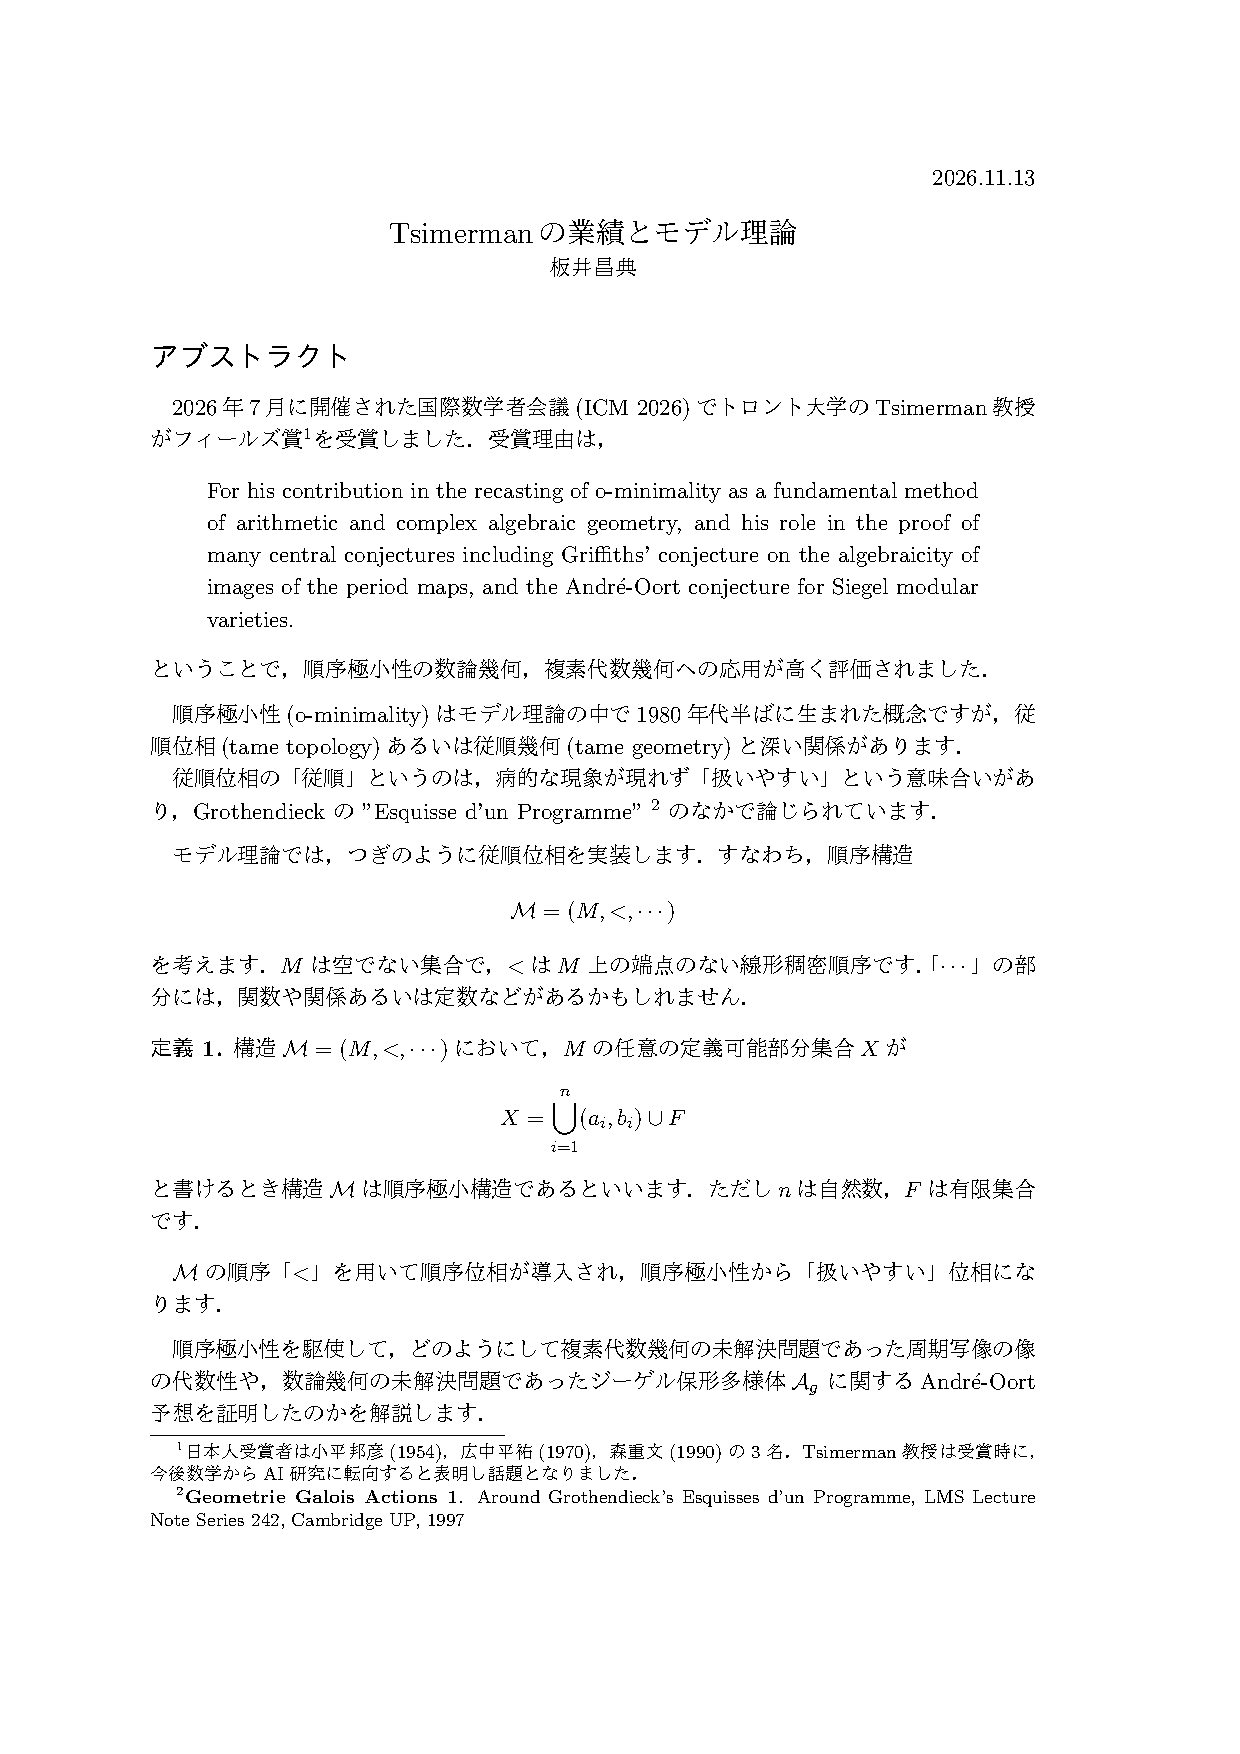
\includepdf[pages=-,fitpaper]{./abstract_itai_2026.pdf}

\end{document}

